\documentclass{beamer}

\mode<presentation> {

% The Beamer class comes with a number of default slide themes
% which change the colors and layouts of slides. Below this is a list
% of all the themes, uncomment each in turn to see what they look like.

\usetheme{Amsterdam}
%\usetheme{default}
%\usetheme{AnnArbor}
%\usetheme{Antibes}
%\usetheme{Bergen}
%\usetheme{Berkeley}
%\usetheme{Berlin}
%\usetheme{Boadilla}
%\usetheme{CambridgeUS}
%\usetheme{Copenhagen}
%\usetheme{Darmstadt}
%\usetheme{Dresden}
%\usetheme{Frankfurt}
%\usetheme{Goettingen}
%\usetheme{Hannover}
%\usetheme{Ilmenau}
%\usetheme{JuanLesPins}
%\usetheme{Luebeck}
%\usetheme{Madrid}
%\usetheme{Malmoe}
%\usetheme{Marburg}
%\usetheme{Montpellier}
%\usetheme{PaloAlto}
%\usetheme{Pittsburgh}
%\usetheme{Rochester}
%\usetheme{Singapore}
%\usetheme{Szeged}
%\usetheme{Warsaw}

% As well as themes, the Beamer class has a number of color themes
% for any slide theme. Uncomment each of these in turn to see how it
% changes the colors of your current slide theme.

%\usecolortheme{albatross}
%\usecolortheme{beaver}
%\usecolortheme{beetle}
%\usecolortheme{crane}
%\usecolortheme{dolphin}
%\usecolortheme{dove}
%\usecolortheme{fly}
%\usecolortheme{lily}
%\usecolortheme{orchid}
%\usecolortheme{rose}
%\usecolortheme{seagull}
%\usecolortheme{seahorse}
%\usecolortheme{whale}
%\usecolortheme{wolverine}

%\setbeamertemplate{footline} % To remove the footer line in all slides uncomment this line
%\setbeamertemplate{footline}[page number] % To replace the footer line in all slides with a simple slide count uncomment this line

%\setbeamertemplate{navigation symbols}{} % To remove the navigation symbols from the bottom of all slides uncomment this line
}

\usepackage{listings}
\usepackage{graphicx} % Allows including images
\usepackage{booktabs} % Allows the use of \toprule, \midrule and \bottomrule in tables
\usepackage[utf8]{inputenc}
\usepackage[english,brazilian]{babel}


%----------------------------------------------------------------------------------------
%	TITLE PAGE
%----------------------------------------------------------------------------------------

\title[Git 101]{Git 101 - An introduction to Git} % The short title appears at the bottom of every slide, the full title is only on the title page

\author{Beraldo Leal} % Your name
\institute[NCC/UNESP] % Your institution as it will appear on the bottom of every slide, may be shorthand to save space
{
Sao Paulo State University - UNESP \\ % Your institution for the title page
\medskip
\textit{beraldo@ncc.unesp.br} % Your email address
}
\date{\today} % Date, can be changed to a custom date

\begin{document}



\begin{frame}
\titlepage % Print the title page as the first slide
\end{frame}

%----------------------------------------------------------------------------------------
%	PRESENTATION SLIDES
%----------------------------------------------------------------------------------------

%------------------------------------------------
\section{Introduction} % Sections can be created in order to organize your presentation into discrete blocks, all sections and subsections are automatically printed in the table of contents as an overview of the talk
%------------------------------------------------

%\subsection{Subsection Example} % A subsection can be created just before a set of slides with a common theme to further break down your presentation into chunks

\frame{\insertsection}

\begin{frame}
\frametitle{What is a Version Control System (VCS) ?}
\begin{itemize}
\item In computer software engineering, revision control is any kind of
practice that tracks and provides control over changes to source code.
\end{itemize}
\end{frame}

\begin{frame}
\frametitle{What is a Version Control System?}
  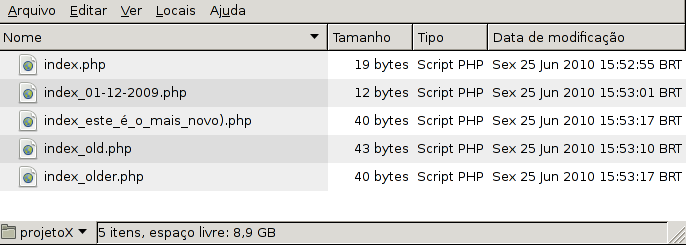
\includegraphics[width=1\textwidth]{imgs/01.png}
\end{frame}

\begin{frame}
\frametitle{History control}
  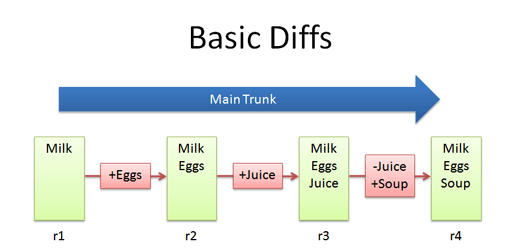
\includegraphics[width=1\textwidth]{imgs/04.png}
\end{frame}

\begin{frame}
\frametitle{What are the types of VCS ?}
\begin{itemize}
\item Based on topology:
  \begin{itemize}
  \item Local;
  \item Centralized;
  \item Distributed;
  \end{itemize}
\end{itemize}
\end{frame}

\begin{frame}
\frametitle{Local}
\begin{center}
  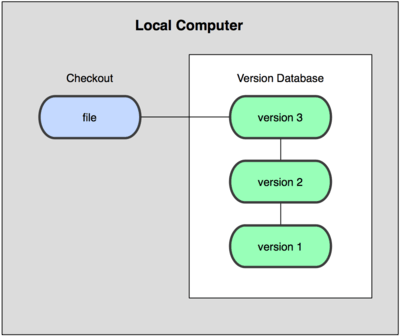
\includegraphics[width=\textwidth,height=0.6\textheight,keepaspectratio]{imgs/local.png}
\end{center}
\end{frame}

\begin{frame}
\frametitle{Centralized}
\begin{center}
  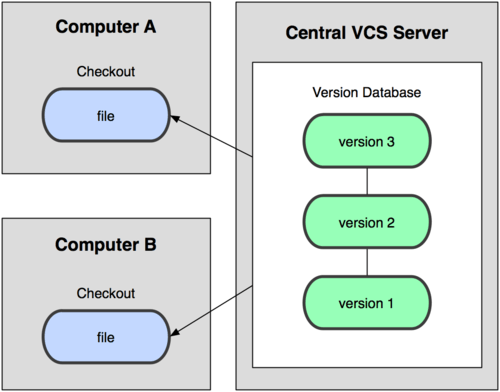
\includegraphics[width=\textwidth,height=0.6\textheight,keepaspectratio]{imgs/centralized.png}
\end{center}
\end{frame}

\begin{frame}
\frametitle{Distributed}
\begin{center}
  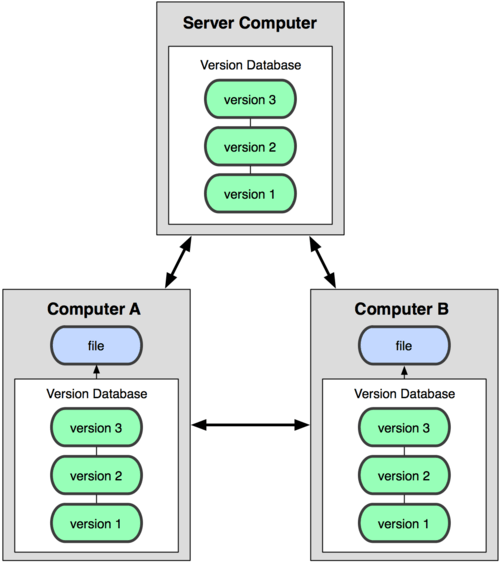
\includegraphics[width=\textwidth,height=0.8\textheight,keepaspectratio]{imgs/distributed.png}
\end{center}
\end{frame}

\begin{frame}
\frametitle{What is Git ?}
\begin{center}
  
\includegraphics[width=0.4\textwidth]{imgs/git-logo.png}
\end{center}
\begin{itemize}
\item Git is a free and open source distributed version control system designed
to handle everything from small to very large projects with speed and
efficiency.
\item by Linus Torvalds (7 April 2005)
\item http://git-scm.com/
\end{itemize}
\end{frame}

\begin{frame}
\frametitle{What is Github ?}
\begin{center}
  
\includegraphics[width=0.3\textwidth]{imgs/github-logo.png}
\end{center}
\begin{itemize}
\item GitHub is a Git repository web-based hosting service which offers all of
the distributed revision control and source code management (SCM) functionality
of Git as well as adding many of its own features.
\item http://www.github.com/
\end{itemize}
\end{frame}

\begin{frame}
\frametitle{Main features of a VCS}
\begin{itemize}
\item History control (versions);
\item Teamwork;
\item Version merge;
\item File locking;
\item Baselines, labels and tags;
\item Branches.
\end{itemize}
\end{frame}

\begin{frame}
\frametitle{Diffs and Patches}
\begin{itemize}
\item diff - the difference between two files;
\item patch - method to apply a diff.
\end{itemize}
\end{frame}

\begin{frame}
\frametitle{Diffs and Patches}
  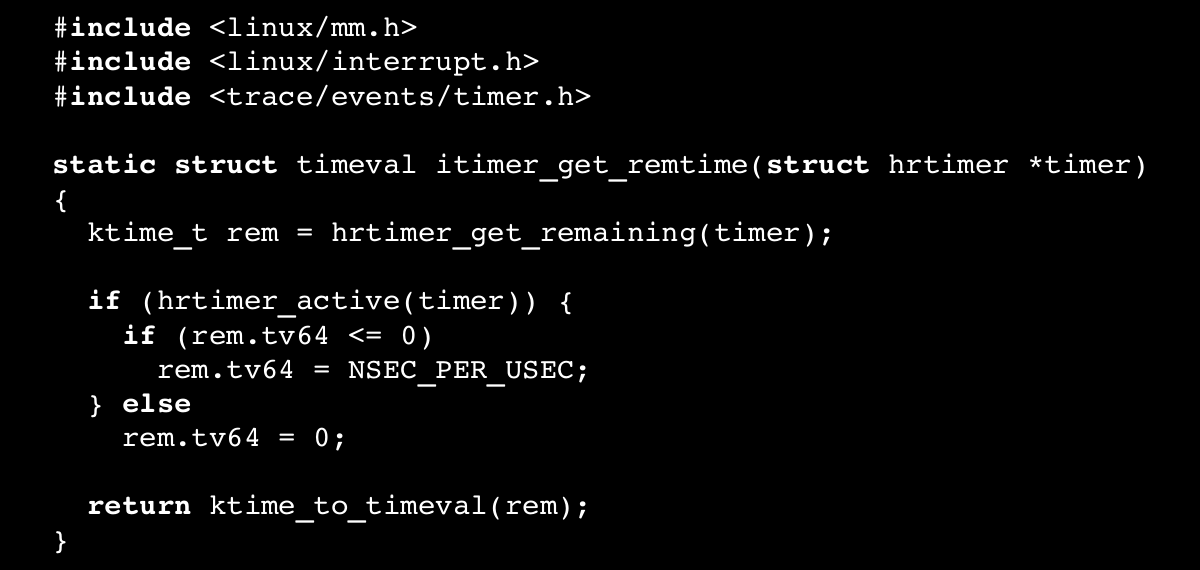
\includegraphics[width=1\textwidth]{imgs/diff-01.png}
\end{frame}

\begin{frame}
\frametitle{Diffs and Patches}
  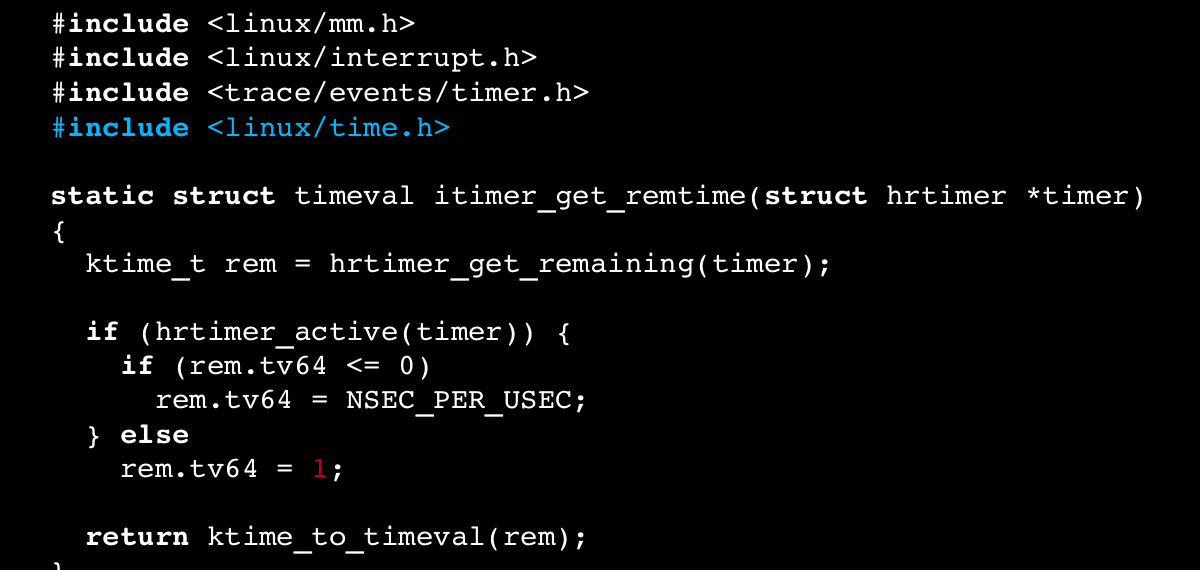
\includegraphics[width=1\textwidth]{imgs/diff-02.png}
\end{frame}

\begin{frame}
\frametitle{Diffs and Patches}
  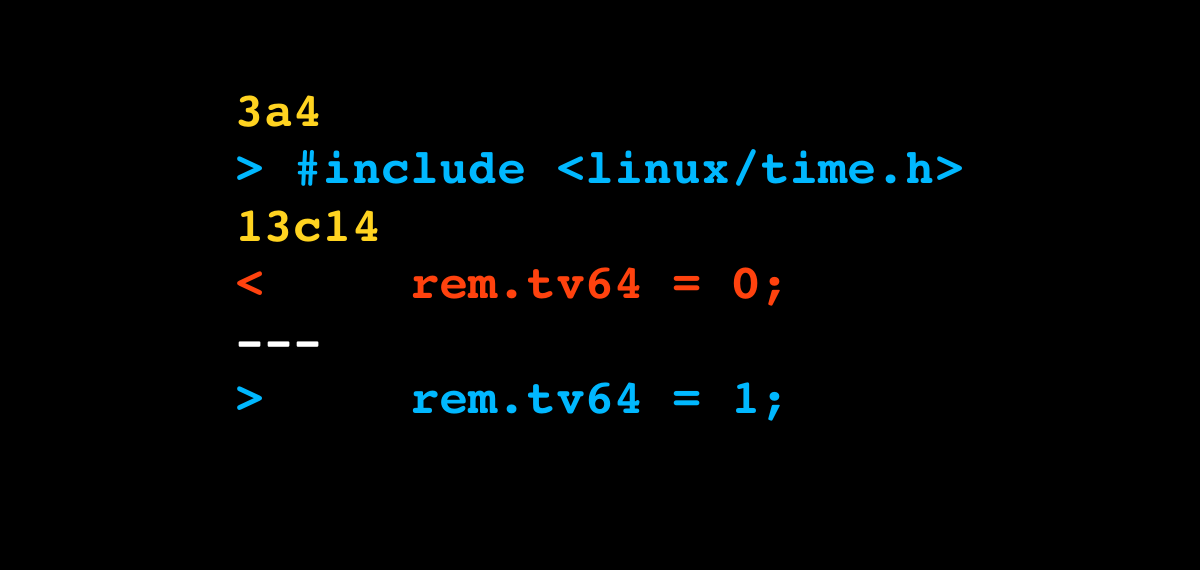
\includegraphics[width=1\textwidth]{imgs/diff-03.png}
\end{frame}

\begin{frame}
\frametitle{Diffs and Patches}
  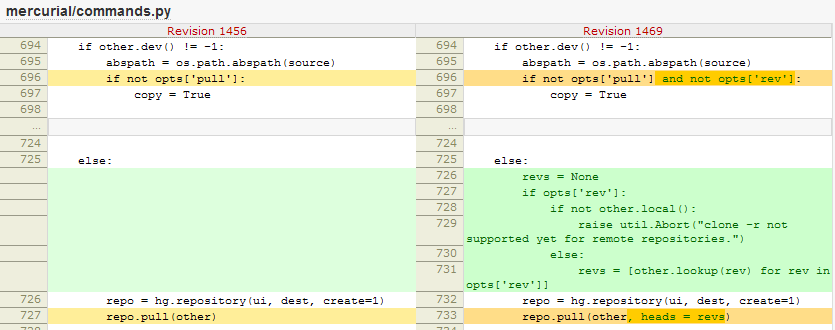
\includegraphics[width=1\textwidth]{imgs/02.png}
\end{frame}

\begin{frame}
\frametitle{Diffs and Patches}
  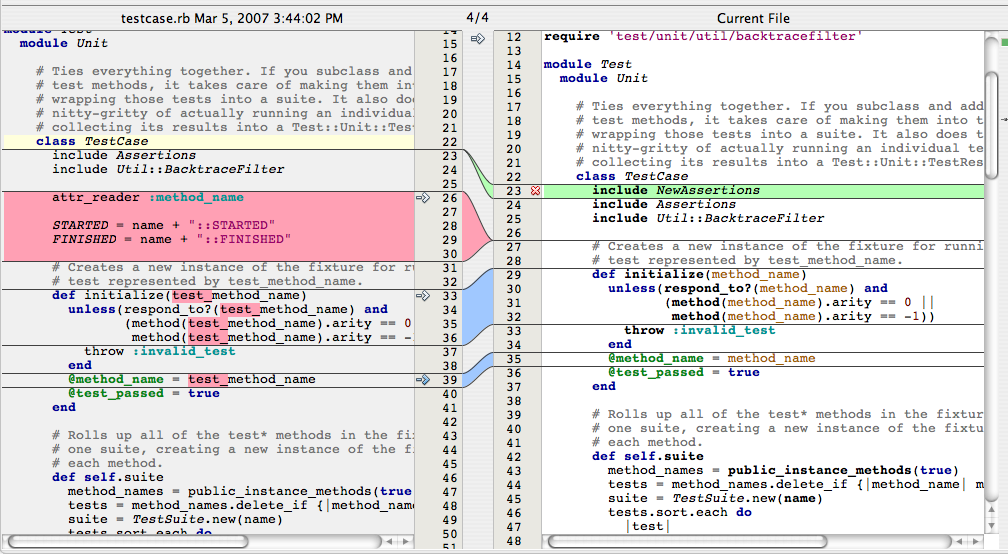
\includegraphics[width=1\textwidth]{imgs/03.png}
\end{frame}

\begin{frame}
\frametitle{Teamwork - Simple scenario}
\begin{center}
  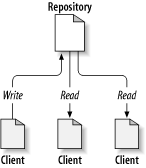
\includegraphics[width=\textwidth,height=0.6\textheight,keepaspectratio]{imgs/screen06.png}
\end{center}
\end{frame}

\begin{frame}
\frametitle{Teamwork - Complex scenario}
\begin{center}
  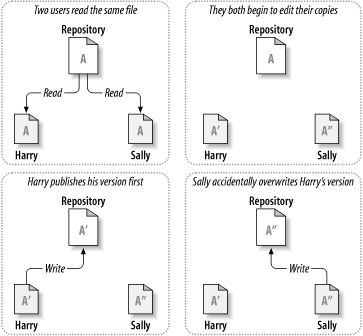
\includegraphics[width=\textwidth,height=0.8\textheight,keepaspectratio]{imgs/screen07.png}
\end{center}
\end{frame}

\section{Git Concepts}

\begin{frame}
\frametitle{Three States}
Commited, modified and staged:
\begin{center}
  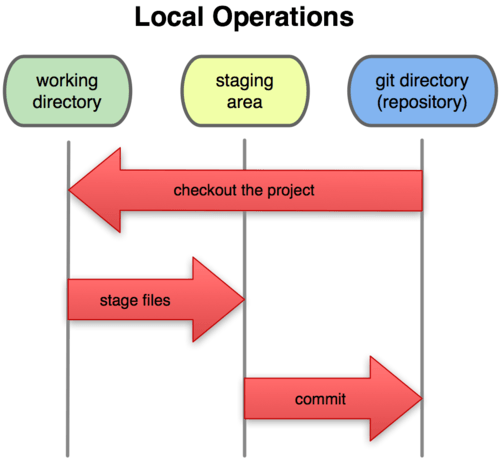
\includegraphics[width=\textwidth,height=0.6\textheight,keepaspectratio]{imgs/states.png}
\end{center}
\end{frame}

\begin{frame}[fragile]
\frametitle{Initial Configuration}
\begin{lstlisting}
$ git config --global user.name "John Doe"
$ git config --global user.email john@doe.com
\end{lstlisting}
\end{frame}

\begin{frame}[fragile]
\frametitle{Your editor}
\begin{lstlisting}
$ git config --global core.editor vim
\end{lstlisting}
\end{frame}

\begin{frame}[fragile]
\frametitle{Starting a repository}
\begin{lstlisting}
$ git init
$ git add *.c
$ git add README
$ git commit -m 'initial project version'
\end{lstlisting}
\end{frame}

\begin{frame}[fragile]
\frametitle{Cloning a repository}
\begin{lstlisting}
$ git clone git@github.com:ncc-unesp/git101.git
\end{lstlisting}
\end{frame}

\begin{frame}
\frametitle{Life cycle}
\begin{center}
  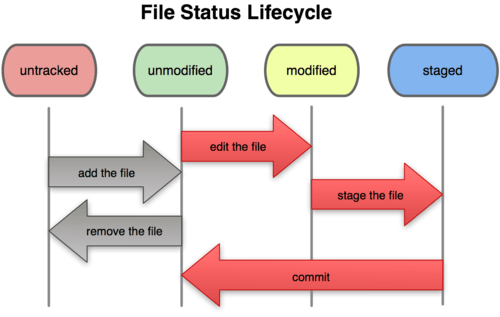
\includegraphics[width=\textwidth,height=0.6\textheight,keepaspectratio]{imgs/life-cycle.png}
\end{center}
\end{frame}

\begin{frame}[fragile]
\frametitle{Checking status}
\begin{lstlisting}
$ git status
\end{lstlisting}
\end{frame}

\begin{frame}[fragile]
\frametitle{Removing files}
\begin{lstlisting}
$ git rm README
\end{lstlisting}
\end{frame}

\begin{frame}[fragile]
\frametitle{Moving files}
\begin{lstlisting}
$ git mv README LEIAME
\end{lstlisting}
\end{frame}

\begin{frame}[fragile]
\frametitle{Ignoring files}
\begin{lstlisting}
$ cat .gitignore
*.[oa]
*~
\end{lstlisting}
\end{frame}

\begin{frame}[fragile]
\frametitle{Visualizing log history}
\begin{lstlisting}
$ git log
$ git log --pretty=oneline
$ git log --pretty=format:"%h - %an, %ar : %s"
\end{lstlisting}
\end{frame}

\section{Branches and tags}
\begin{frame}
\frametitle{Simple scenario}
\begin{center}
  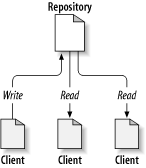
\includegraphics[width=\textwidth,height=0.6\textheight,keepaspectratio]{imgs/screen06.png}
\end{center}
\end{frame}


\section{Advanced}

\begin{frame}
\frametitle{Fixing merge conflicts}
\begin{itemize}
\item Can manually edit the files;
\item Use a merge tool (like diffmerge);
\end{itemize}
\end{frame}

%------------------------------------------------

\begin{frame}
\frametitle{Questions?}

Beraldo Leal - beraldo@ncc.unesp.br
\end{frame}

%----------------------------------------------------------------------------------------

\end{document} 
